\graphicspath{{./figs/chap2/}} % graphics location for this chapter
\chapter{Experimental Setup and Device Fabrication}\label{chap:two}
In this chapter the techniques needed in order to fabricate \ac{2D} transistors
are introduced and explained. Basic techniques such as the exfoliation of atomically thin \acp{TMD} crystals 
to more advanced techniques such as \ac{vdW} assembly of structures using various transfer methods are explored
in great detail. In addition, more general processes related to the fabrication of semiconductor devices
are explained as well. 

\section{Sample Preparation}\label{sec:sample_prep}
\subsection{Synthesis of Crystal Material}\label{subsec:crystal_synthesis}

\section{Preparation of Atomically Thin Two-Dimensional Materials}\label{sec:prep_of_samples}
\subsection{Exfoliation of Atomically Thin Materials}\label{subsec:exfoliation}
\subsection{Characterization of Atomically Thin Materials}\label{subsec:exfoliation_characterization}
\begin{figure}[ht]
    \centering
    \subfloat[]{
        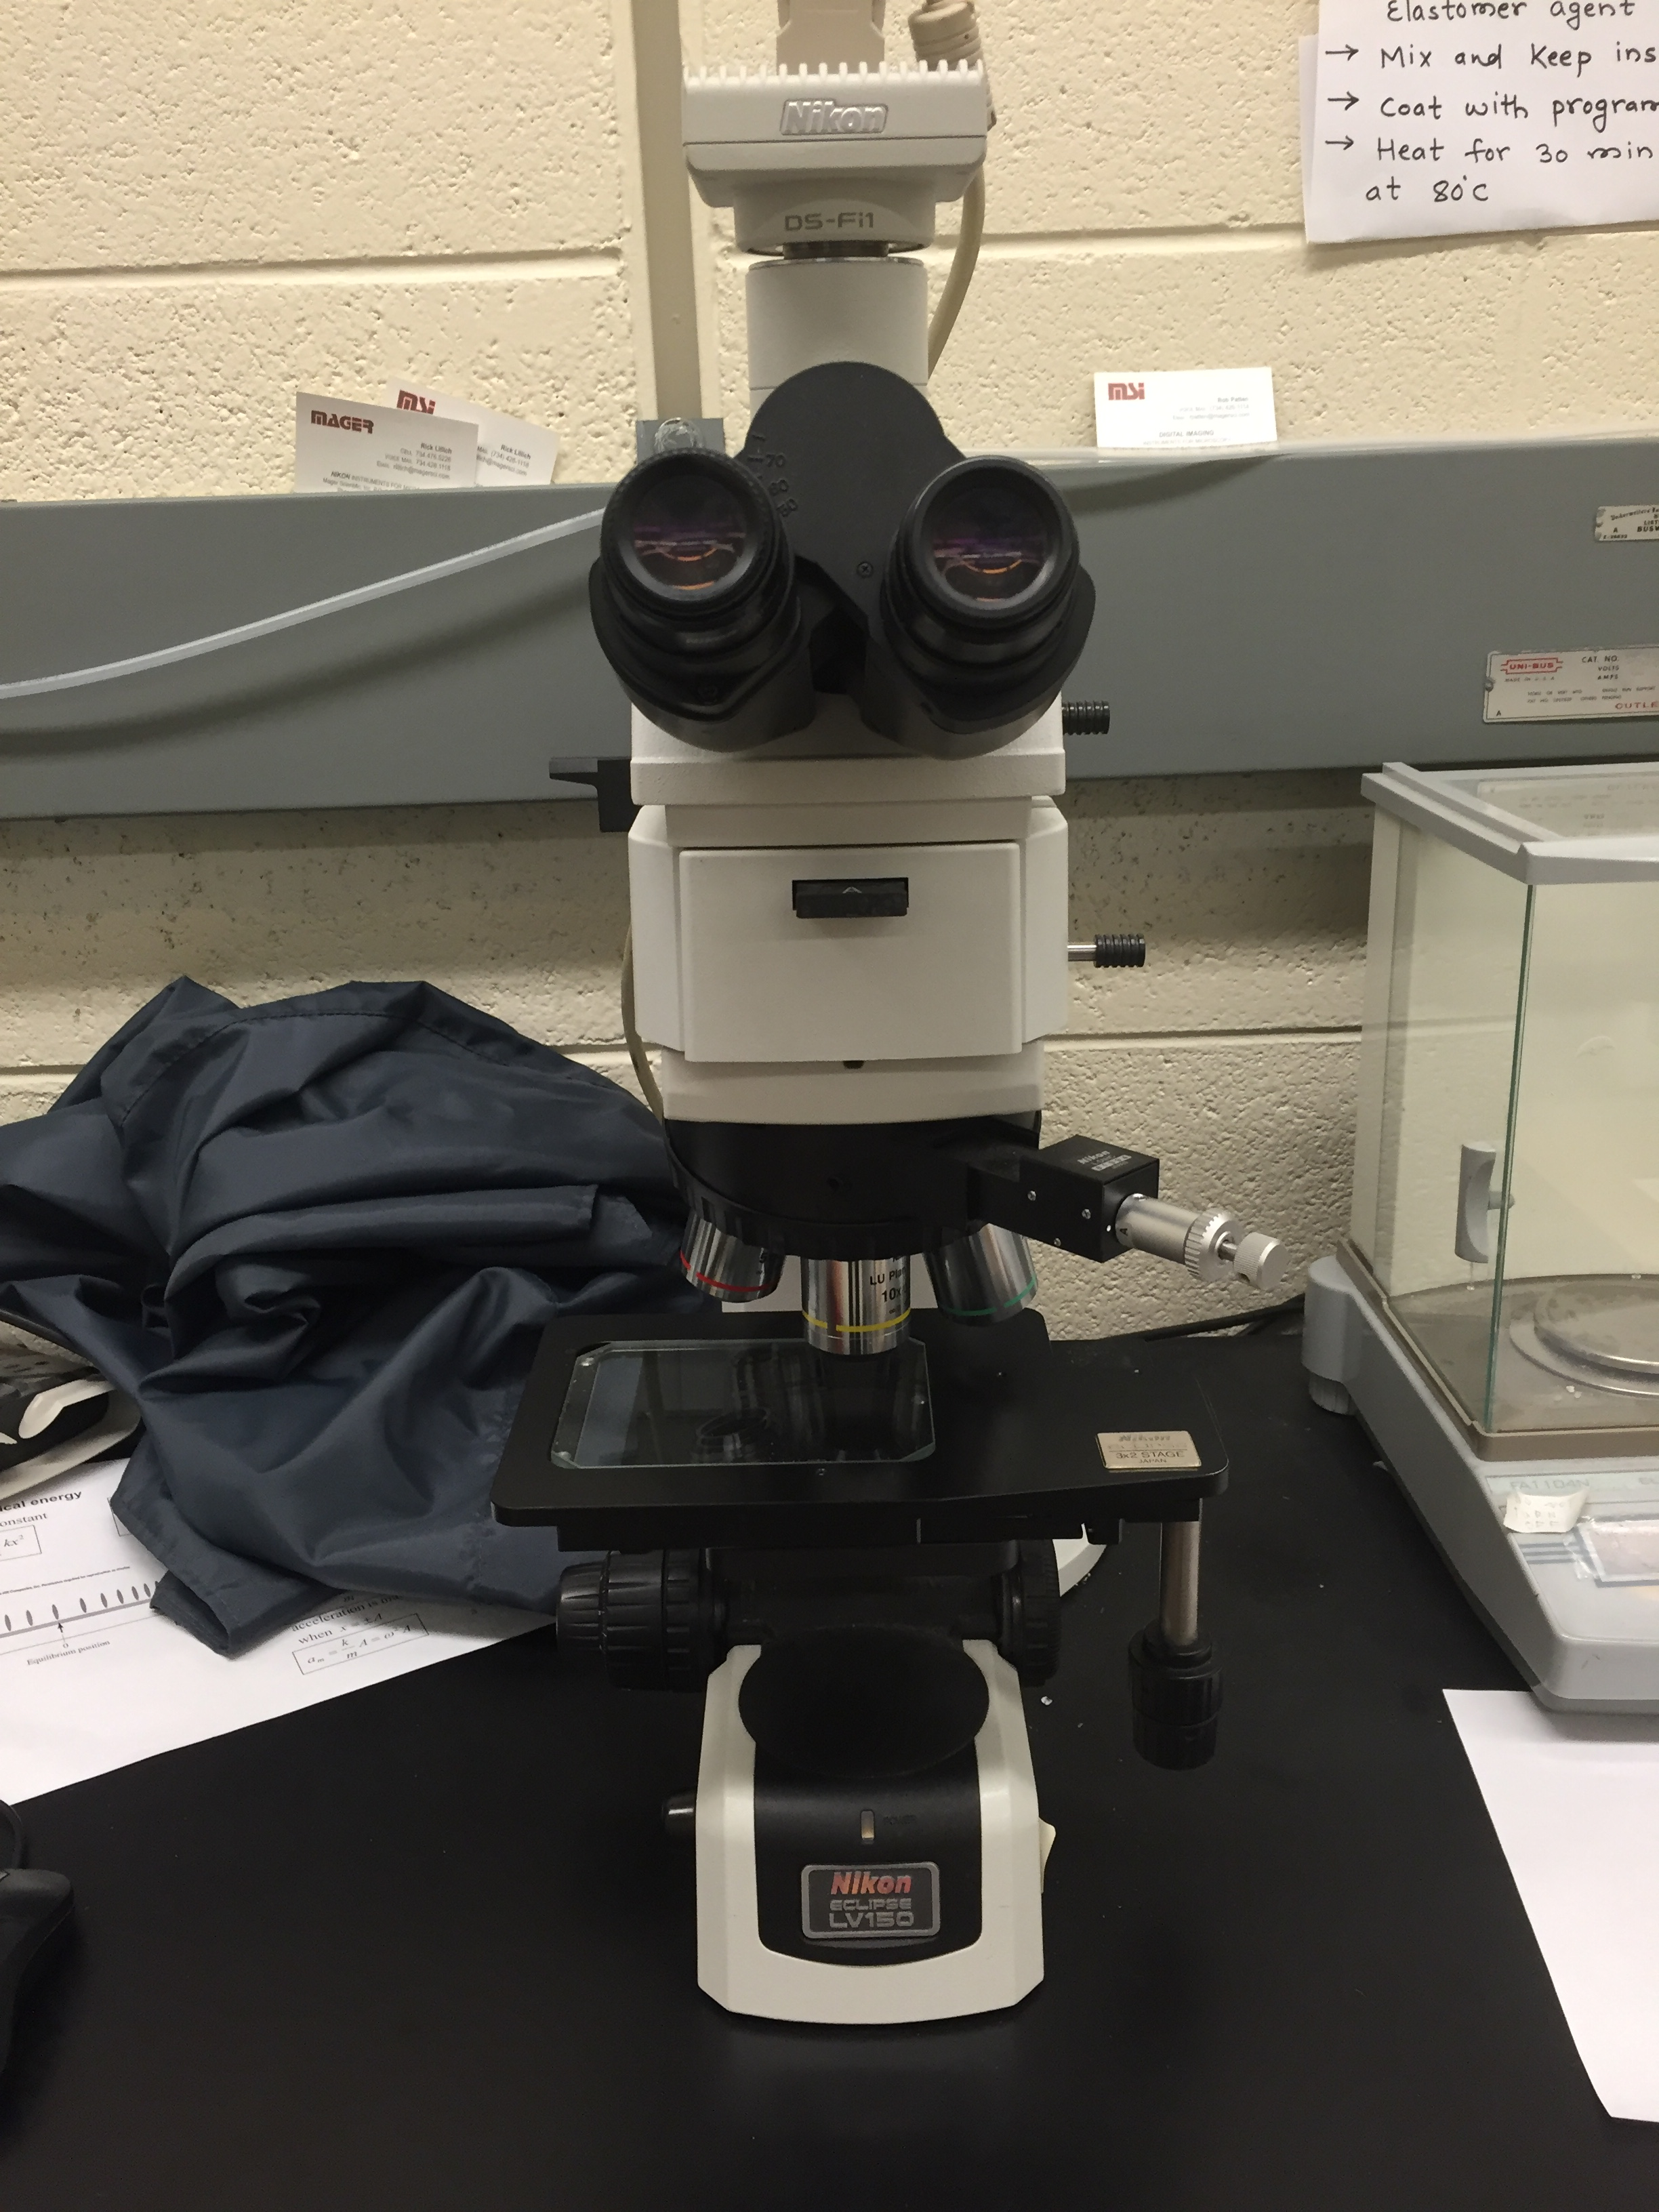
\includegraphics[height=5cm,width=3.5cm]{optical_microscope_front_view}
        \label{fig:optical_microscope_front_view}
    }
    \qquad
    \subfloat[]{
        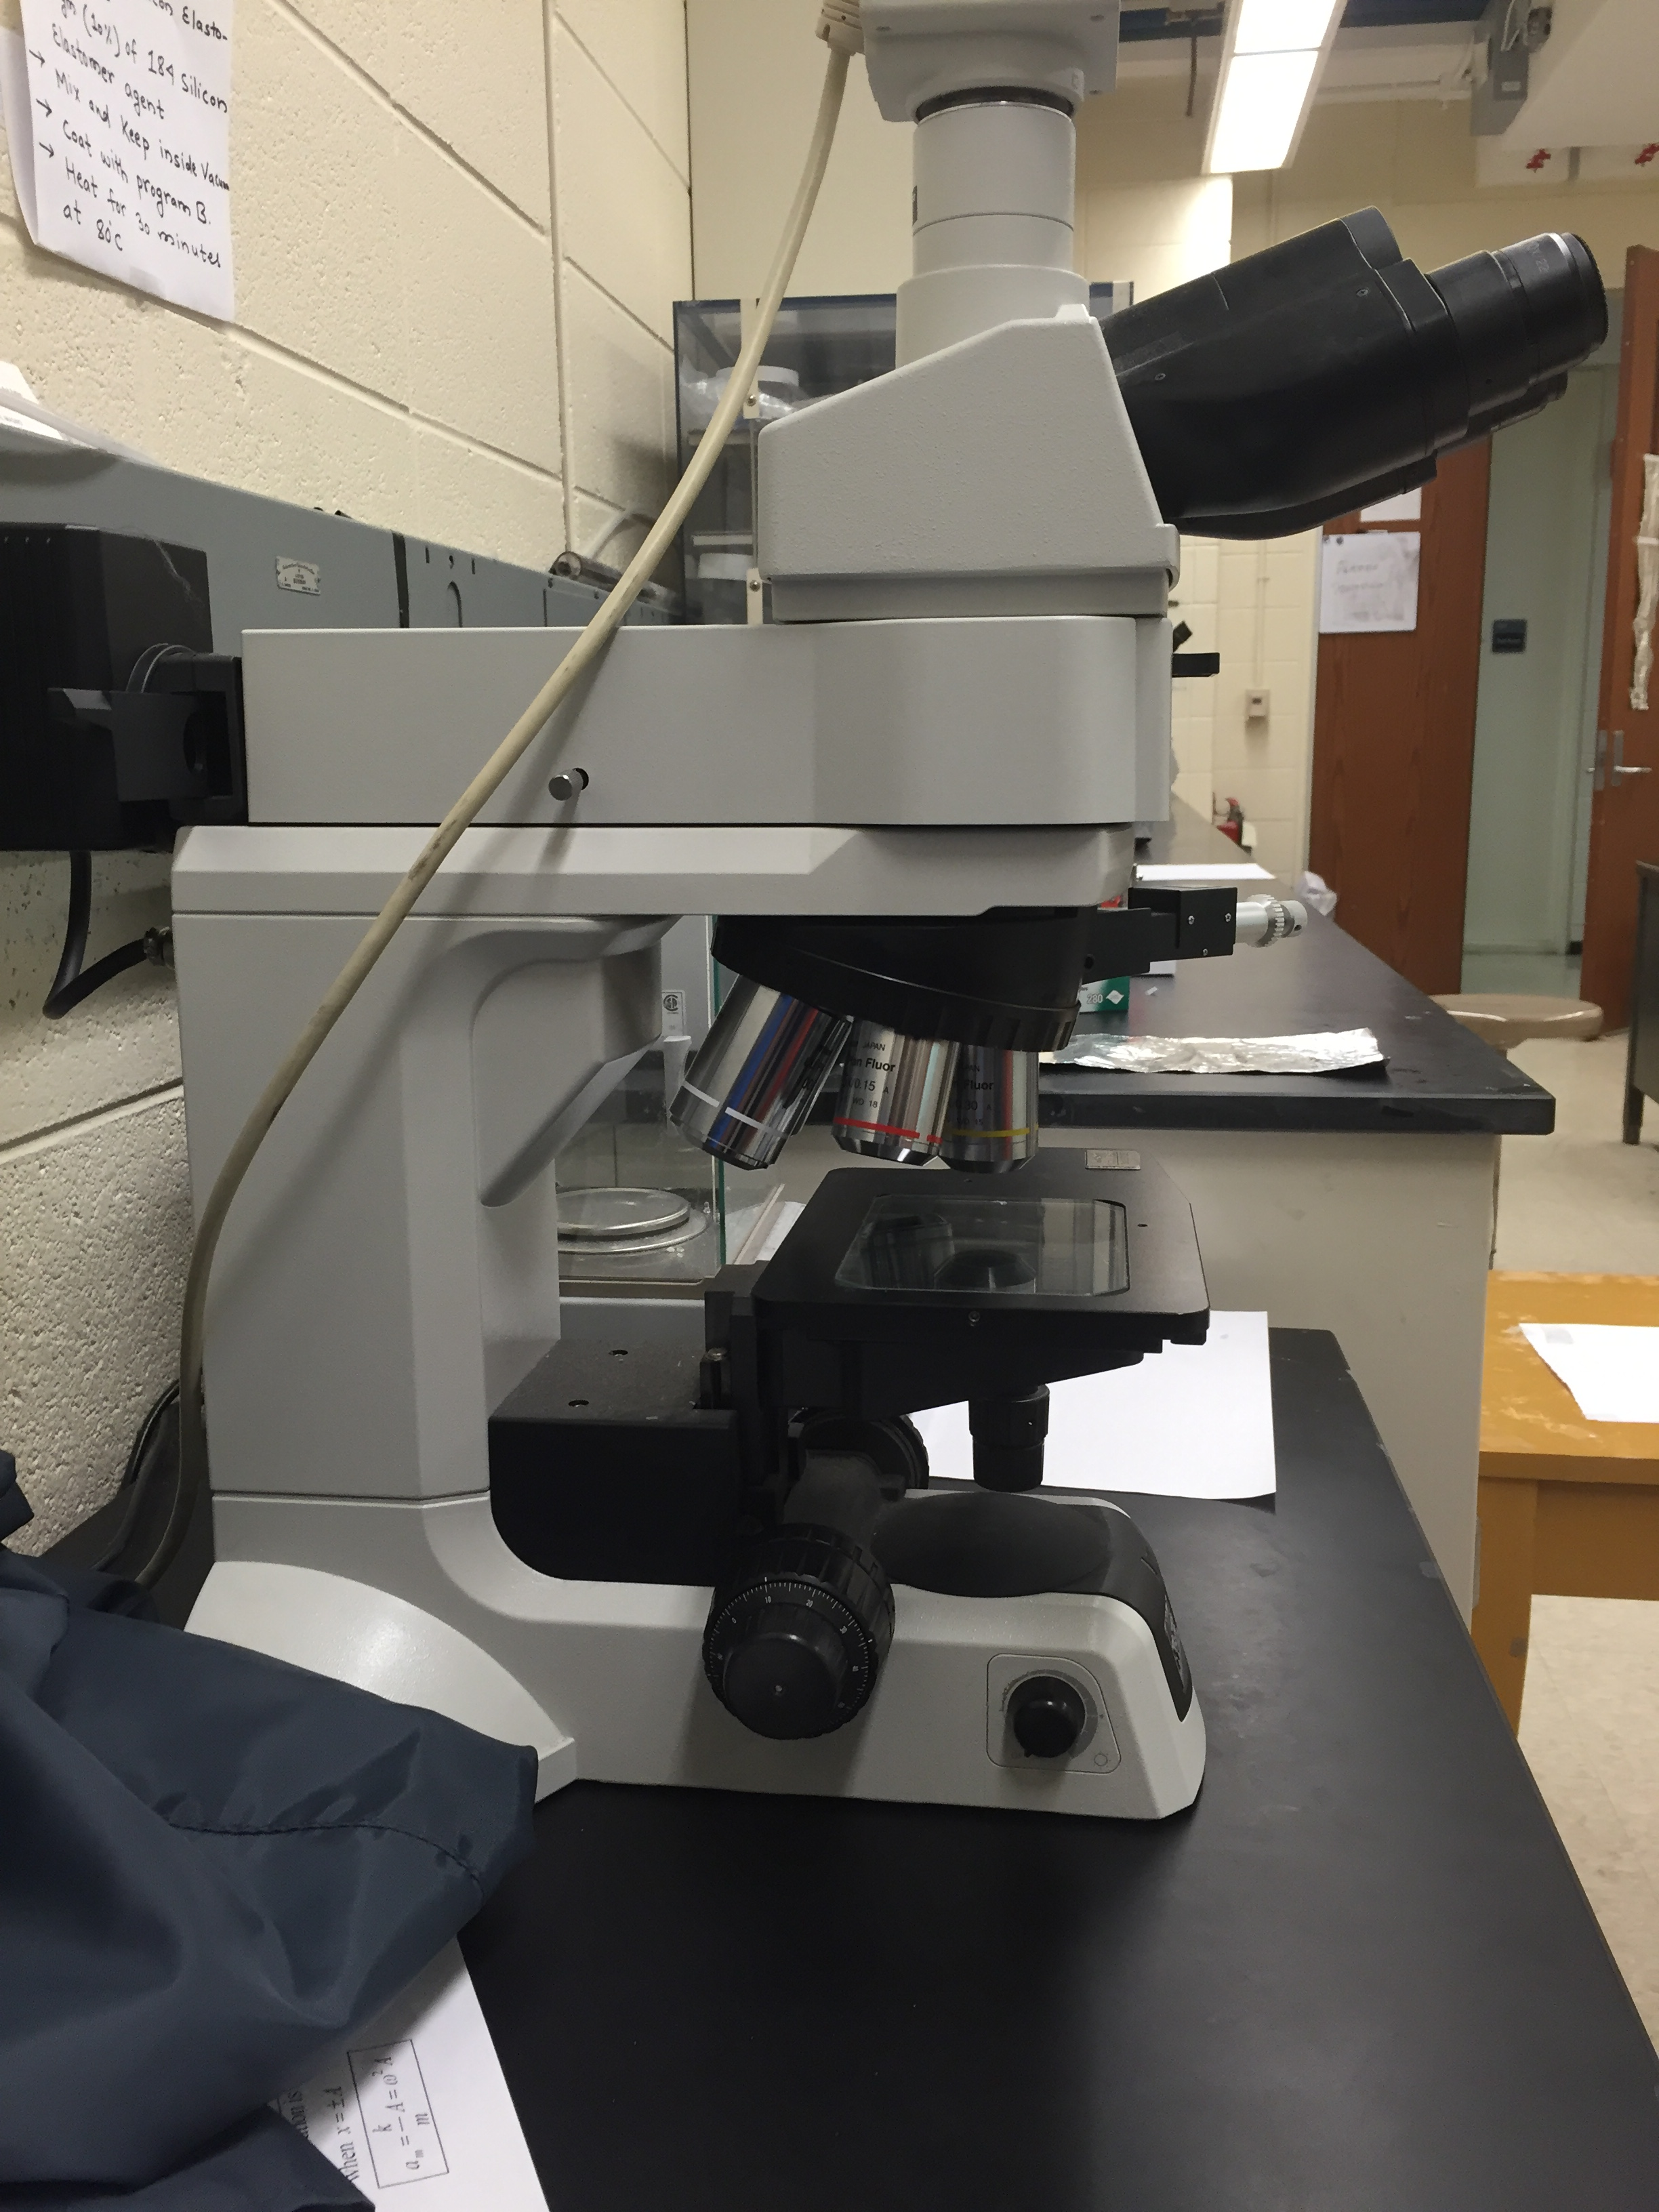
\includegraphics[height=5cm,width=3.5cm]{optical_microscope_side_view}
        \label{fig:optical_microscope_side_view}
    }
    \caption[Optical microscope setup]{\protect\subref{fig:optical_microscope_front_view} Optical microscope front view. \protect\subref{fig:optical_microscope_side_view} Optical microscope size view.}
\end{figure}
\begin{figure}[ht]
    \centering  
    \subfloat[]{
        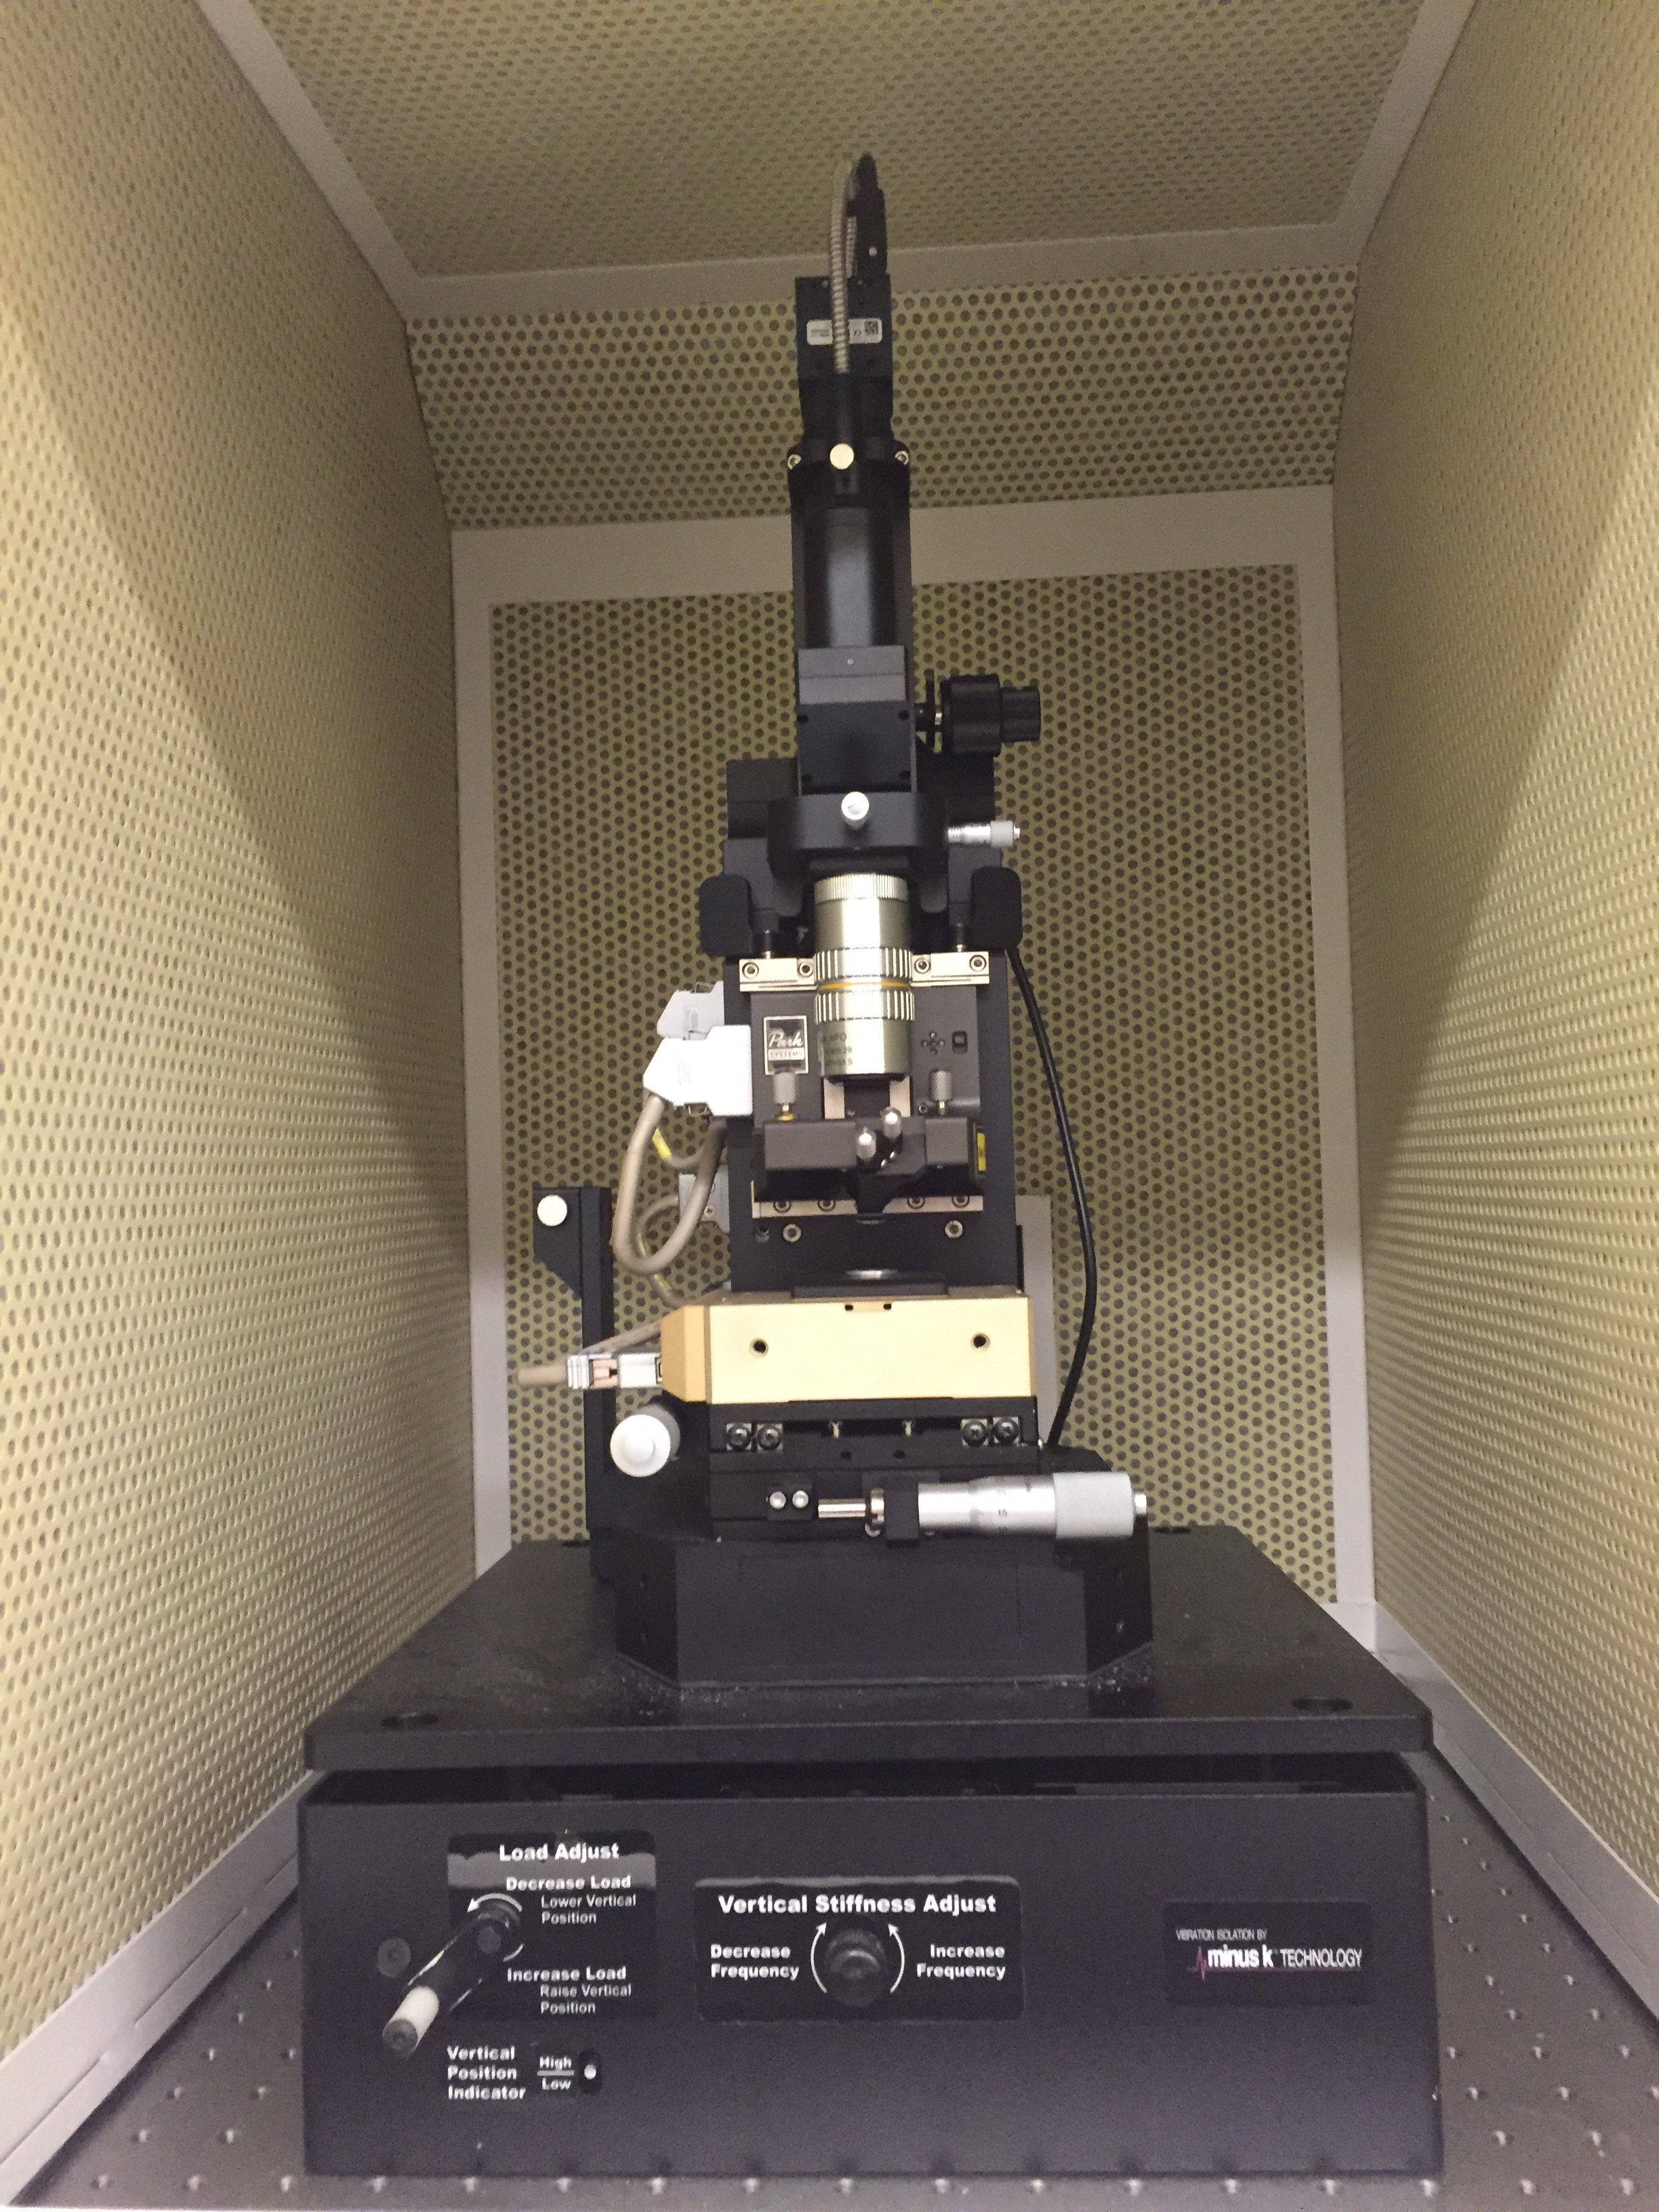
\includegraphics[height=4cm,width=4cm]{AFM_front_view}
        \label{fig:afm_front_view}
    }
    \qquad
    \subfloat[]{
        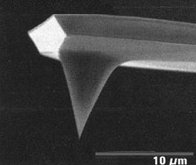
\includegraphics[height=4cm,width=4cm]{AFM_tip}
        \label{fig:AFM_tip}
    }
    \caption[Diagram of atomic force microscope setup and cantilever]{\protect\subref{fig:afm_front_view} Front view of \acs{AFM} setup. \protect\subref{fig:AFM_tip} AFM cantilever tip.}
\end{figure}

\section{Stacking and Assembly of Two-Dimensional Materials}\label{sec:transfer}
\subsection{PDMS Film Preparation}\label{subsec:pdms_prep}
\subsection{PDMS Transfer Method}\label{subsec:pdms_transfer}
\subsection{PC Film Preparation}\label{subsec:pc_prep}
\subsection{Wet PC Transfer Method}\label{subsec:_wet_pc_transfer}
\subsection{Dry PC Transfer and Sequential Pickup Methods}\label{subsec:dry_pc_transfer}

\section{Doping Methods}\label{sec:chemical_doping}
\subsection{Doping Methods: Benzyl Viologen}\label{subsec:doping_bv}
\subsection{Doping Methods: Polymer Electrolyte}\label{subsec:doping_pe}

\section{General Fabrication Processes}\label{sec:fab_processes}
\subsection{Electron Beam Lithography}\label{subsec:ebl}
\begin{figure}[ht]
    \centering
    \includegraphics[height=4cm,width=7cm]{SEM}
    \caption[Scanning electron microscope]{Control panel and electron beam writing system using a \acs{SEM}.}
\end{figure} 
\subsection{Photolithography}\label{subsec:photo_lithography}
\subsection{Metal Deposition}\label{subsec:metal_deposition}
\subsection{Lift Off}\label{subsec:lift_off}
\subsection{Sample Annealing}\label{subsec:annealing}
